\documentclass[11pt]{article}

\usepackage[hidelinks]{hyperref}

\usepackage{graphicx}
\usepackage[export]{adjustbox}
\graphicspath{{images/}}
\usepackage{float}

\usepackage{amsmath}
% for more advanced math equations

\usepackage{parskip}
% enter a vertical space between paragraphs and skip the indentation

\usepackage{geometry}
\geometry{
	a4paper
}

\usepackage{polyglossia}
\setdefaultlanguage[variant=modern]{greek}
\setotherlanguage{english}
\newfontfamily\greekfont{Open Sans Light}
\newfontfamily\greekfonttt{Inconsolata}
\newfontfamily\englishfont{Open Sans Light}
\newfontfamily\englishfonttt{Inconsolata}

\usepackage{listings}
\lstset{
    frame=single,
    breaklines=true,
    postbreak=\raisebox{0ex}[0ex][0ex]{\ensuremath{\color{blue}\hookrightarrow\space}}
}

\usepackage{datetime2}
% sudo dnf install texlive-datetime2-english
% sudo dnf install texlive-datetime2-greek
\DTMnewdatestyle{monthyear}{%
    \renewcommand*{\DTMdisplaydate}[4]{\DTMgreekmonthname{##2}, ##1}%
    \renewcommand*{\DTMDisplaydate}{\DTMdisplaydate}%
}
\DTMsetdatestyle{monthyear}
\renewcommand*{\DTMgreekmonthname}[1]{%
    \ifcase#1
    \or
    Ιανουάριος%
    \or
    Φεβρουάριος%
    \or
    Μάρτιος%
    \or
    Απρίλιος%
    \or
    Μάιος%
    \or
    Ιούνιος%
    \or
    Ιούλιος%
    \or
    Αύγουστος%
    \or
    Σεπτέμβριος%
    \or
    Οκτόβριος%
    \or
    Νοέμβριος%
    \or
    Δεκέμβριος%
    \fi
}

\usepackage{siunitx}

\title{Προσέγγιση Συνάρτησης δύο Διαστάσεων\\με Χρήση Νευρωνικού Δικτύου}
\date{\DTMtoday}
\author{Γκαντίδης Χρήστος 56483 \\ email: \href{mailto:chrigkan@ee.duth.gr}{chrigkan@ee.duth.gr}}

\begin{document}
\pagenumbering{gobble}
% don't number first page
\maketitle
\newpage

\tableofcontents
\newpage

\pagenumbering{arabic}

\section{Εισαγωγή}

Στο πρόβλημα της προσέγγισης μιας συνάρτησης με χρήση ενός Νευρωνικού Δικτύου\textendash ΝΔ (Neural Network), σου δίνεται μια συνάρτηση δύο διαστάσεων, και πρέπει χρησιμοποιώντας έναν μικρό αριθμό από τιμές της συνάρτησης αυτής στο επίπεδο, να εκπαιδεύσεις ένα νευρωνικό δίκτυο, ώστε να συμπεριφέρεται ως η συνάρτηση που σου δίνεται.

Για την συγκεκριμένη περίπτωση, η συνάρτηση που πρέπει να προσεγγιστεί είναι η

\begin{equation*}
	f(x, y)=sin(\pi x) + con(\pi y),\quad x, y \in [-1, 1]
\end{equation*}

Για την εκπαίδευση του ΝΔ χρησιμοποιούνται 200 ζεύγη συντεταγμένων $(x, y)$ και οι αντίστοιχες τιμές της συνάρτησης στις συντεταγμένες αυτές. Οι συντεταγμένες επιλέγονται τυχαία, ακολουθώντας ομοιόμορφη κατανομή, από ένα σύνολο $50^2=2500$ συντεταγμένων, οι οποίες είναι γραμμικά και ομοιόμορφα διατεταγμένες στο επίπεδο $xy$.

\section{Δομή του Νευρωνικού Δικτύου}

\subsection{Είσοδος}

Στο επίπεδο της εισόδου του ΝΔ, υπάρχουν δύο νευρώνες. Ο ένας νευρώνας δέχεται την τιμή του $x$ και ο άλλος την τιμή του $y$ από ένα ζεύγος συντεταγμένων, στο οποίο προσεγγίζεται η τιμή της συνάρτησης με το ΝΔ.

\subsection{Κρυφά Επίπεδα}

Στην συγκεκριμένη περίπτωση, χρησιμοποιείται ένα κρυφό επίπεδο με 10 νευρώνες. Η χρήση λιγότερων νευρώνων στο κρυφό επίπεδο οδηγεί σε underfitting, με αποτέλεσμα το ΝΔ να μην μπορεί να προσεγγίσει τον μεγάλο βαθμό ελευθερίας της συνάρτησης. Η χρήση περισσότερων νευρώνων στο κρυφό επίπεδο ή η χρήση περισσότερων κρυφών επιπέδων οδηγεί σε overfitting, με αποτέλεσμα το ΝΔ να τα πηγαίνει πολύ καλά στα δεδομένα εκπαίδευσης (training set), αλλά να έχει πολύ κακή συμπεριφορά στα δεδομένα ελέγχου (test set), καθώς το πλήθος των δεδομένων εκπαίδευσης δεν είναι αρκετά μεγάλο ώστε να εκπαιδευτούν αρκετά καλά όλοι οι νευρώνες.

\subsection{Έξοδος}

Στο επίπεδο της εξόδου του ΝΔ, υπάρχει μόνο ένας νευρώνας, του οποίου η τιμή εξόδου αναπαριστά την προσεγγιστική τιμή που υπολόγισε το ΝΔ για την συγκεκριμένη είσοδο.

\section{Αλγόριθμος Εκπαίδευσης}

Για της εκπαίδευση του ΝΔ χρησιμοποιείται η συνάρτηση του MATLAB \texttt{trainlm} η οποία υλοποιεί έναν αλγόριθμο μάθησης με οπισθοδιάδοση (backpropagation), ανανεώνοντας τα βάρη ενεργοποίησης των νευρώνων και των σταθερών τιμών (bias units), όπως περιγράφηκε από τους Levenberg\textendash Marquardt.

\section{Συνάρτηση Ενεργοποίησης}

Για την ενεργοποίηση του κρυφού επιπέδου από τις εξόδους του επιπέδου εισόδου, χρησιμοποιείται η συνάρτηση ενεργοποίησης του MATLAB \texttt{tansig} που είναι μια σιγμοειδής καμπύλη υπερβολικής εφαπτομένης.

Για την ενεργοποίηση του επιπέδου εξόδου από τις εξόδους του κρυφού επιπέδου χρησιμοποιείται η συνάρτηση ενεργοποίησης του MATLAB \texttt{purelin} που είναι μια αμιγώς γραμμική συνάρτηση.

\section{Αποτελέσματα}

Για την δοκιμή της απόδοσης του ΝΔ επιλέγονται 85 ζεύγη συντεταγμένων $(x, y)$ και οι αντίστοιχες τιμές της συνάρτησης στις συντεταγμένες αυτές. Οι συντεταγμένες επιλέγονται τυχαία, ακολουθώντας ομοιόμορφη κατανομή, από το αρχικό σύνολο των $2500$ συντεταγμένων, και καμία τους δεν ανήκει στο αρχικό σετ εκπαίδευσης του ΝΔ, ώστε να μην υπάρχει πλεονέκτημα υπέρ του ΝΔ, να μην εξεταστεί δηλαδή το ΝΔ πάνω σε συντεταγμένες για τις οποίες έχει εκπαιδευτεί.

Το πλήθος των συντεταγμένων δοκιμής έχει επιλεγεί ώστε να έχει έναν λόγο 30\% προς 70\% με τα δεδομένα εκπαίδευσης.

Η απόδοση του ΝΔ καθορίζεται από το τελικό μέσο τετραγωνικό κανονικοποιημένο σφάλμα στην έξοδο του δικτύου. Η τάξη του σφάλματος είναι της τάξης του $10^{-4}$.

\begin{lstlisting}
Mean Squared Error: 0.000171
\end{lstlisting}

\begin{figure}[H]
\makebox[\textwidth]{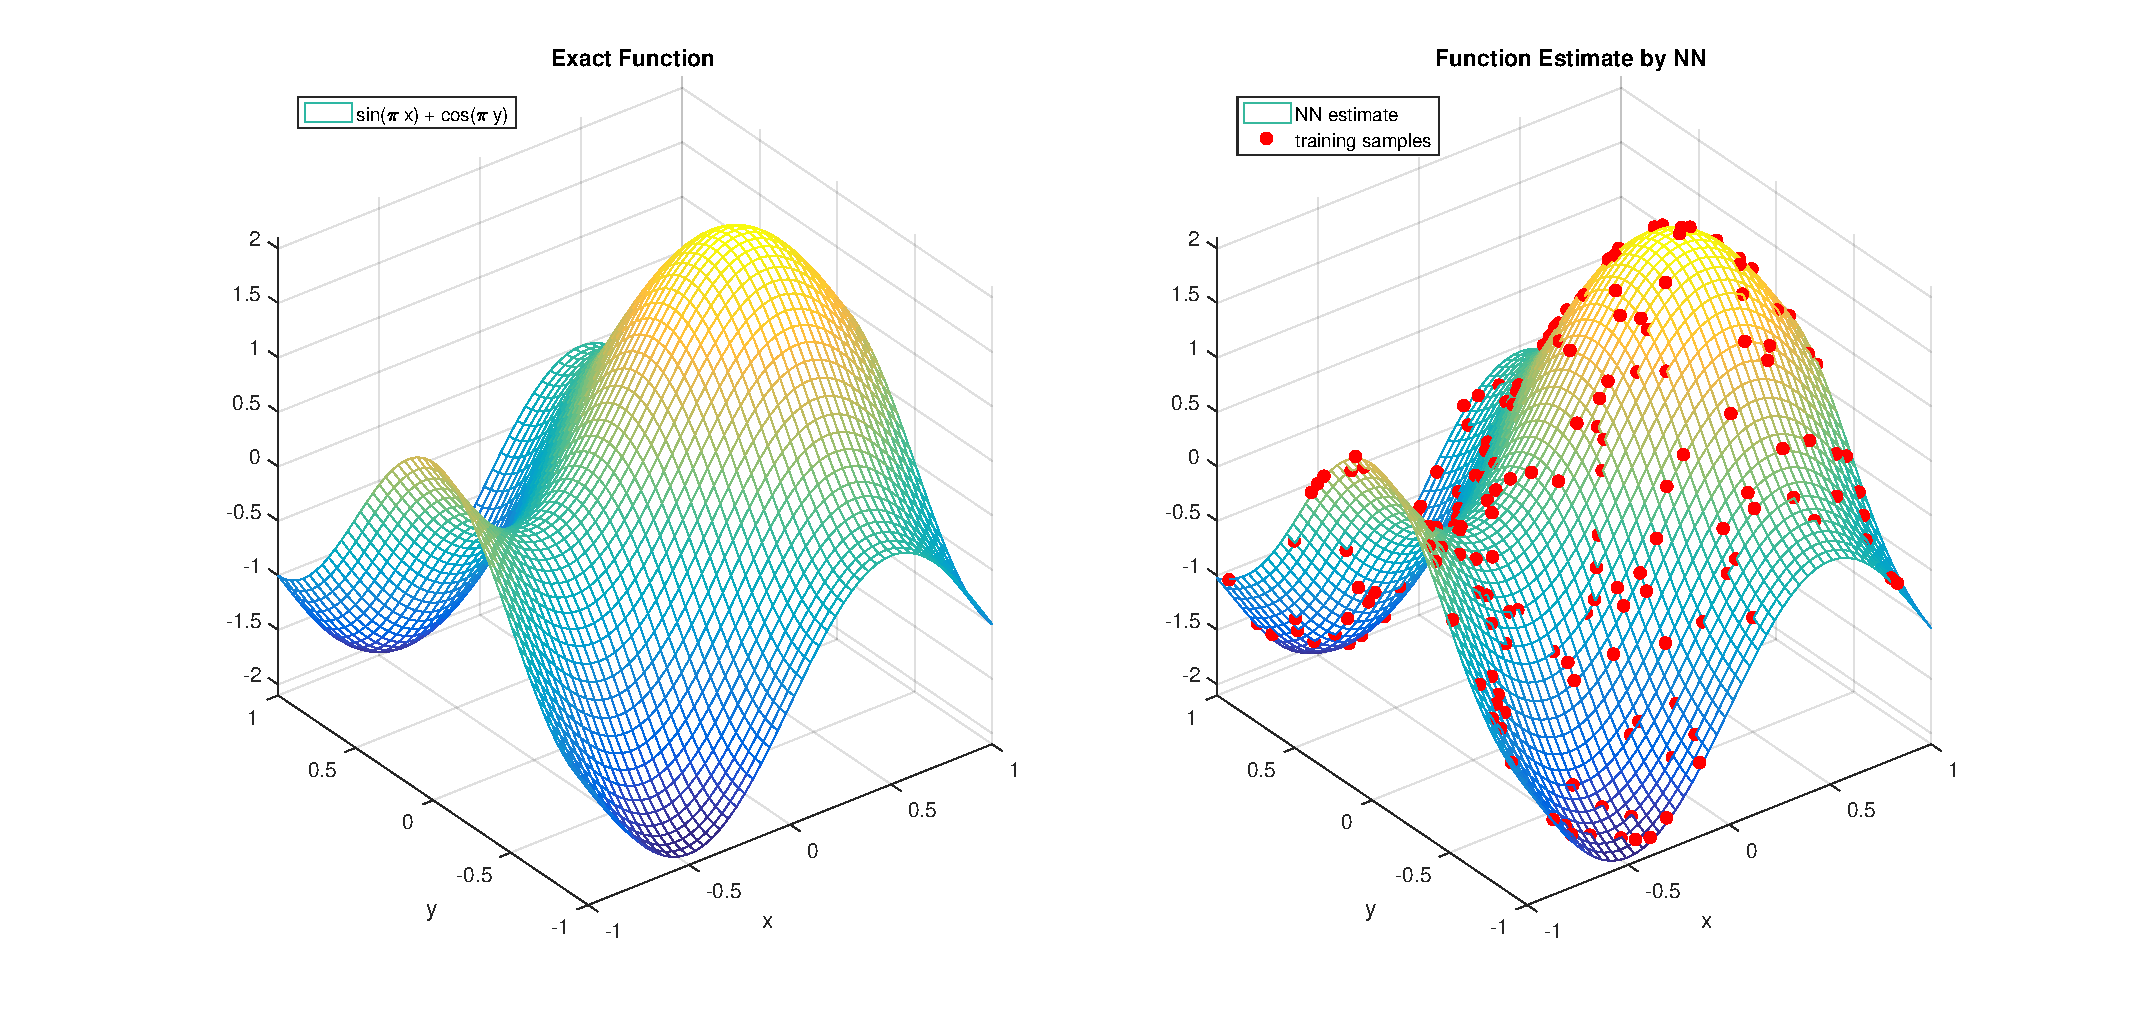
\includegraphics[width=\paperwidth]{fun_approx}}
\caption{Προσέγγιση Συνάρτησης με Νευρωνικό Δίκτυο}
\end{figure}

\end{document}
